\chapter{Multipletes de momento angular, movimiento radial y escalera del oscilador}

\section{Dependencia angular de la función de onda}

Una partícula en un campo de fuerza central tiene una coordenada radial y dos coordenadas angulares. Clásicamente,
\begin{equation}
\mathbf L=\mathbf r\times\mathbf p
\end{equation}
se conserva como vector. Su dirección determina el plano de la órbita, aunque esta no tiene por qué ser circular.

En mecánica cuántica, la partícula se describe mediante
\begin{equation}
\Psi=\Psi(r,\theta,\phi),
\end{equation}
y el momento angular está relacionado con la dependencia de esta función de onda respecto de los ángulos.

En dos dimensiones solo hay una componente del momento angular: el generador de las rotaciones alrededor del eje perpendicular al plano:
\begin{equation}
L_z=-i\hbar\frac{\partial}{\partial\theta}.
\end{equation}
Una autofunción con autovalor \(\hbar\ell\) satisface
\begin{equation}
-i\hbar\frac{\partial}{\partial\theta}\psi(r,\theta)
=\hbar\ell\,\psi(r,\theta).
\end{equation}
La coordenada \(r\) es un parámetro espectador en esta ecuación. La solución tiene la forma
\begin{equation}
\psi(r,\theta)=\chi(r)e^{i\ell\theta}.
\end{equation}
Para una función de onda orbital ordinaria de valor único, volver al mismo punto tras \(\theta\to\theta+2\pi\) exige que \(\ell\) sea un entero. El factor radial \(\chi(r)\) puede afectar a la energía, pero no afecta a este autovalor del momento angular.

El análogo tridimensional separa la dependencia radial de las funciones definidas sobre la esfera:
\begin{equation}
\Psi(r,\theta,\phi)=R(r)Y_{\ell m}(\theta,\phi).
\end{equation}
Las funciones \(Y_{\ell m}\) son armónicos esféricos. Aquí no necesitaremos sus fórmulas explícitas. Las rotaciones actúan sobre el factor angular, mientras que la función radial permanece inalterada.

\section{Multipletes de momento angular finitos}

Las componentes del momento angular satisfacen
\begin{equation}
\begin{aligned}
[L_x,L_y]&=i\hbar L_z,\\
[L_y,L_z]&=i\hbar L_x,\\
[L_z,L_x]&=i\hbar L_y.
\end{aligned}
\end{equation}
Elijamos autoestados de \(L_z\),
\begin{equation}
L_z|\ell,m\rangle=\hbar m\,|\ell,m\rangle,
\end{equation}
y definamos
\begin{equation}
L_\pm=L_x\pm iL_y.
\end{equation}
Los conmutadores
\begin{equation}
[L_z,L_\pm]=\pm\hbar L_\pm
\end{equation}
dan
\begin{align}
L_z\bigl(L_\pm|\ell,m\rangle\bigr)
&=\bigl(L_\pm L_z+[L_z,L_\pm]\bigr)|\ell,m\rangle \\
&=\hbar(m\pm1)L_\pm|\ell,m\rangle.
\end{align}
Así, \(L_+\) aumenta \(m\) en una unidad y \(L_-\) lo disminuye en una unidad, salvo que el vector resultante sea nulo.

En un multiplete finito hay un estado de valor máximo y otro de valor mínimo:
\begin{equation}
L_+|\ell,\ell\rangle=0,
\qquad
L_-|\ell,-\ell\rangle=0.
\end{equation}
Las direcciones \(+z\) y \(-z\) están relacionadas por una rotación, por lo que el espectro finito es simétrico respecto de cero. Por tanto, sus valores son
\begin{equation}
m=-\ell,-\ell+1,\ldots,\ell-1,\ell,
\end{equation}
y el número de estados es
\begin{equation}
2\ell+1.
\end{equation}
Como los valores vecinos difieren en una unidad, los extremos pueden ser enteros o semienteros. Los armónicos esféricos orbitales ordinarios realizan el caso entero; el álgebra abstracta del momento angular también admite multipletes semienteros.

\begin{classroomqa}
\lecturetimestamp{00:16:12}
\audiencequestion{¿Podría un multiplete de momento angular contener infinitos estados?}
\lecturerresponse{Es una posibilidad que se puede considerar, pero no hará falta aquí. En general, el momento angular aumenta la energía si se mantienen fijas las demás características del estado; por ello, los estados con momento angular infinito no son pertinentes al estudiar estados de energía finita.}
\end{classroomqa}

\section{\texorpdfstring{\(L^2\)}{El valor común de }}

El operador que mide el cuadrado de la magnitud del momento angular es
\begin{equation}
L^2=L_x^2+L_y^2+L_z^2.
\end{equation}
El producto ordenado de los operadores escalera es
\begin{align}
L_-L_+
&=(L_x-iL_y)(L_x+iL_y) \\
&=L_x^2+L_y^2+i[L_x,L_y] \\
&=L_x^2+L_y^2-\hbar L_z.
\end{align}
En consecuencia,
\begin{equation}
L^2=L_z^2+\hbar L_z+L_-L_+.
\end{equation}
Apliquemos esta identidad al estado de valor máximo. Como \(L_+|\ell,\ell\rangle=0\),
\begin{align}
L^2|\ell,\ell\rangle
&=\left(L_z^2+\hbar L_z+L_-L_+\right)|\ell,\ell\rangle \\
&=\hbar^2\left(\ell^2+\ell\right)|\ell,\ell\rangle,
\end{align}
y, por tanto,
\begin{equation}
L^2|\ell,\ell\rangle
=\hbar^2\ell(\ell+1)|\ell,\ell\rangle.
\end{equation}
El cuadrado de la magnitud no es \(\hbar^2\ell^2\). El término adicional se debe a la no conmutatividad de las componentes del momento angular.

Este mismo valor corresponde a todos los estados del multiplete, no solo al de valor máximo.

\begin{classroomqa}
\lecturetimestamp{00:26:08}
\audiencequestion{¿Qué demuestra exactamente el ejercicio sobre la igualdad del valor de \(L^2\) para los demás estados?}
\lecturerresponse{Demuestre que \(L^2\) conmuta con cada componente del momento angular y, por tanto, con \(L_-\). Luego, haga pasar \(L^2\) a través de \(L_-\): si el estado de valor máximo tiene autovalor \(\hbar^2\ell(\ell+1)\), el estado inmediatamente inferior tiene el mismo autovalor. Al repetir el argumento, ese valor se conserva a lo largo de toda la escalera.}
\end{classroomqa}

En efecto,
\begin{equation}
[L^2,L_i]=0,
\qquad i=x,y,z,
\end{equation}
por lo que
\begin{equation}
[L^2,L_\pm]=0.
\end{equation}
Por ejemplo,
\begin{align}
L^2\bigl(L_-|\ell,\ell\rangle\bigr)
&=L_-L^2|\ell,\ell\rangle \\
&=\hbar^2\ell(\ell+1)L_-|\ell,\ell\rangle.
\end{align}
Al continuar hacia abajo se obtiene
\begin{equation}
L^2|\ell,m\rangle
=\hbar^2\ell(\ell+1)|\ell,m\rangle
\end{equation}
para todo \(m=-\ell,\ldots,\ell\).

El orden inverso da una factorización equivalente:
\begin{align}
L_+L_-
&=(L_x+iL_y)(L_x-iL_y) \\
&=L_x^2+L_y^2-i[L_x,L_y] \\
&=L_x^2+L_y^2+\hbar L_z,
\end{align}
y, por tanto,
\begin{equation}
L^2=L_z^2-\hbar L_z+L_+L_-.
\end{equation}

\begin{classroomqa}
\lecturetimestamp{00:32:05}
\audiencequestion{¿Se puede factorizar \(L_x^2+L_y^2\) en el orden inverso usando \(L_+L_-\)?}
\lecturerresponse{Sí. El signo del término \(L_z\) cambia. Con ese orden, aplique la identidad al estado de valor mínimo, que es anulado por \(L_-\), en vez de aplicarla al estado de valor máximo. Se obtiene el mismo autovalor, \(\hbar^2\ell(\ell+1)\).}
\end{classroomqa}

Por tanto, los armónicos esféricos satisfacen
\begin{align}
L^2Y_{\ell m}
&=\hbar^2\ell(\ell+1)Y_{\ell m}, \\
L_zY_{\ell m}
&=\hbar m\,Y_{\ell m}.
\end{align}
Para cada valor orbital \(\ell=0,1,2,\ldots\), hay \(2\ell+1\) funciones, etiquetadas por \(m=-\ell,\ldots,\ell\).

Para un potencial central,
\begin{equation}
[H,L_i]=0.
\end{equation}
Si se mantienen fijos un autoestado de energía radial y \(\ell\), cambiar \(m\) mediante \(L_\pm\) no modifica la energía. Por tanto, cada uno de esos autoestados radiales genera un multiplete magnético de dimensión \(2\ell+1\).

A continuación se muestra la escalera orbital entera.\footnote{El diagrama se reconstruyó a partir del esquema del multiplete y de las identidades de los operadores que aparecen en \(00{:}35{:}53\) del video de la clase.}

\begin{figure}[htbp]
\centering
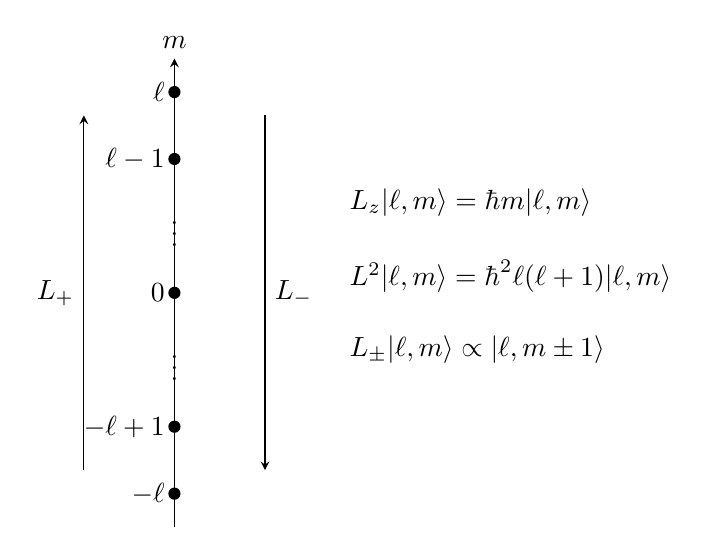
\begin{tikzpicture}[x=1cm,y=0.85cm,>=stealth]
\draw[->] (0,-3.5) -- (0,3.5) node[above] {$m$};

\fill (0,3) circle (2.2pt);
\fill (0,2) circle (2.2pt);
\fill (0,0) circle (2.2pt);
\fill (0,-2) circle (2.2pt);
\fill (0,-3) circle (2.2pt);

\node[left] at (0,3) {$\ell$};
\node[left] at (0,2) {$\ell-1$};
\node[left] at (0,0) {$0$};
\node[left] at (0,-2) {$-\ell+1$};
\node[left] at (0,-3) {$-\ell$};

\node at (0,1) {$\vdots$};
\node at (0,-1) {$\vdots$};

\draw[->] (-1.15,-2.65) -- (-1.15,2.65)
node[midway,left] {$L_+$};
\draw[->] (1.15,2.65) -- (1.15,-2.65)
node[midway,right] {$L_-$};

\node[anchor=west] at (2.1,1.35)
{$L_z|\ell,m\rangle=\hbar m|\ell,m\rangle$};
\node[anchor=west] at (2.1,0.25)
{$L^2|\ell,m\rangle=\hbar^2\ell(\ell+1)|\ell,m\rangle$};
\node[anchor=west] at (2.1,-0.85)
{$L_\pm|\ell,m\rangle\propto|\ell,m\pm1\rangle$};
\end{tikzpicture}
\caption{Un multiplete entero de momento angular orbital. \(L_+\) y \(L_-\) cambian \(m\) en una unidad, mientras que \(L^2\) se mantiene igual a \(\hbar^2\ell(\ell+1)\) en todo el multiplete.}
\lectureframe{00:35:53}
\end{figure}

\section{El problema de la fuerza central}

Consideremos
\begin{equation}
H=\frac{\mathbf p^2}{2m}+V(r),
\end{equation}
donde \(V\) depende únicamente de la distancia al origen. La simetría rotacional implica la conservación del momento angular. Clásicamente, \(\mathbf L\) tiene magnitud y dirección fijas, de modo que la órbita permanece en un plano perpendicular a \(\mathbf L\). La órbita no tiene por qué ser circular ni siquiera cerrada.

Elijamos las coordenadas de modo que ese plano orbital clásico sea el plano \(xy\), y descompongamos el momento en sus componentes radial y tangencial:
\begin{equation}
\mathbf p^2=p_r^2+p_\theta^2.
\end{equation}
Como la magnitud del momento angular es
\begin{equation}
L=r p_\theta,
\end{equation}
la contribución tangencial se puede escribir como
\begin{equation}
p_\theta^2=\frac{L^2}{r^2}.
\end{equation}
El hamiltoniano queda
\begin{equation}
H=\frac{p_r^2}{2m}+\frac{L^2}{2mr^2}+V(r).
\end{equation}
Para un valor fijo de \(L\), este es un problema unidimensional en la coordenada radial, con potencial efectivo
\begin{equation}
V_{\mathrm{eff}}(r)=\frac{L^2}{2mr^2}+V(r).
\end{equation}
A continuación se muestra en la pizarra el hamiltoniano radial.\footnote{Fotograma de referencia: \texttt{\detokenize{lecture_03_frame_02.png}}, video de la clase en \(00{:}47{:}15\).}

\begin{figure}[htbp]
\centering
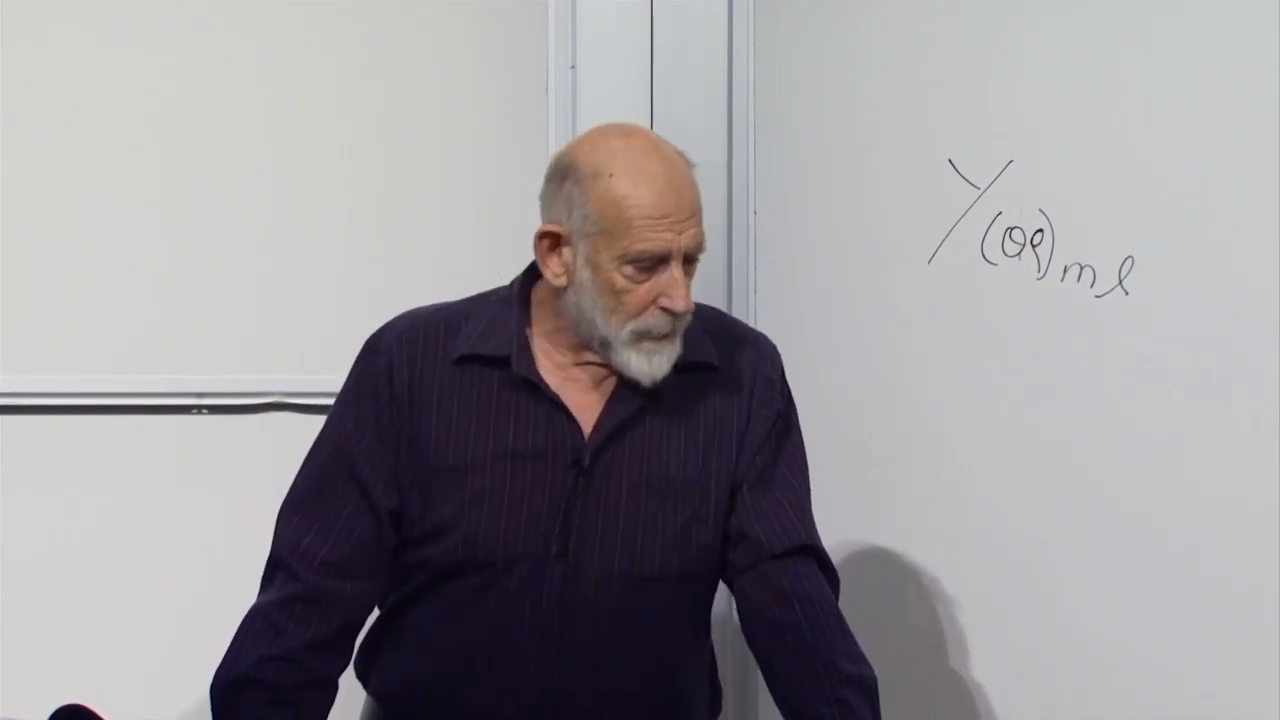
\includegraphics[width=0.9\linewidth]{lecture_03_frame_02.png}
\caption{Para un momento angular clásico fijo, el hamiltoniano radial contiene la energía cinética radial, el término centrífugo \(L^2/(2mr^2)\) y el potencial central \(V(r)\).}
\lectureframe{00:47:15}
\end{figure}

El término \(1/r^2\) es la barrera centrífuga. Aumenta cuando la partícula se acerca al origen, por lo que la fuerza asociada apunta hacia afuera. Para las atracciones de tipo Coulomb que estamos tratando, una trayectoria con \(L\neq0\) gira alrededor del centro en vez de llegar a él. Cuando \(L=0\), la barrera desaparece.

Para el potencial de Coulomb atractivo,
\begin{equation}
V(r)=-\frac{\kappa}{r},
\end{equation}
el término centrífugo domina a distancias pequeñas \(r\), mientras que el término de Coulomb decrece más lentamente y domina a distancias grandes \(r\). Si \(L\neq0\), la suma tiene un mínimo. El movimiento en ese mínimo tiene radio constante y, por tanto, es circular. El movimiento ligado por encima del mínimo y por debajo del umbral de escape oscila entre un radio mínimo y uno máximo; en el problema de Coulomb, estas son las oscilaciones radiales de una órbita elíptica.

\section{La ecuación radial reducida}

En mecánica cuántica, la parte angular de un estado con momento angular orbital definido es un armónico esférico. Escribamos el estado separado como
\begin{equation}
\Psi_{n_r\ell m}(r,\theta,\phi)
=\frac{u_{n_r\ell}(r)}{r}\,
Y_{\ell m}(\theta,\phi).
\end{equation}
El operador angular \(L^2\) tiene el autovalor
\begin{equation}
L^2Y_{\ell m}
=\hbar^2\ell(\ell+1)Y_{\ell m}.
\end{equation}
Para un par fijo \(n_r,\ell\), abreviemos \(u_{n_r\ell}(r)\) como \(u(r)\). La ecuación que queda para la función radial reducida es
\begin{equation}
\begin{aligned}
&-\frac{\hbar^2}{2m}\frac{d^2u}{dr^2}
+\frac{\hbar^2\ell(\ell+1)}{2mr^2}u(r)\\
&\qquad+V(r)u(r)=E_{n_r\ell}\,u(r).
\end{aligned}
\end{equation}

\editorialnote{\(u=rR\) es la función radial reducida que se utiliza en la ecuación unidimensional de derivadas segundas pura. Así, el término \(\psi(r)\) de la ecuación mostrada en la clase corresponde a \(u(r)\), mientras que el factor radial ordinario en \(\Psi=R(r)Y_{\ell m}\) es \(R=u/r\). Esta convención evita tratar \(-i\hbar\,d/dr\) como un operador de momento radial hermítico por sí solo en el espacio de Hilbert radial tridimensional.}

A continuación se muestra en la pizarra la ecuación radial reducida.\footnote{Fotograma de referencia: \texttt{\detokenize{lecture_03_frame_03.png}}, video de la clase en \(00{:}54{:}32\).}

\begin{figure}[htbp]
\centering
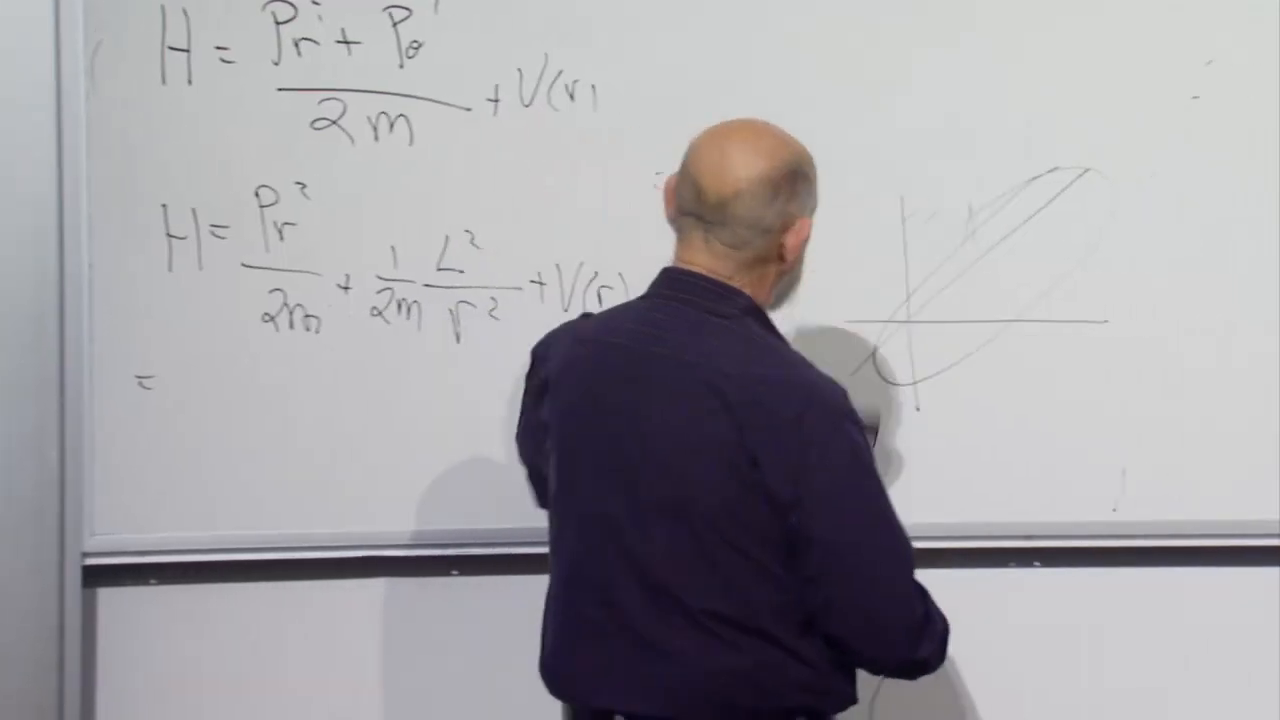
\includegraphics[width=0.9\linewidth]{lecture_03_frame_03.png}
\caption{Para un valor fijo de \(\ell\), la función de onda radial reducida satisface una ecuación unidimensional de Schr\"odinger con un término centrífugo proporcional a \(\ell(\ell+1)/r^2\).}
\lectureframe{00:54:32}
\end{figure}

La estructura angular tridimensional queda condensada en el parámetro \(\ell\). El número cuántico magnético \(m\) no aparece en la ecuación radial.

\begin{classroomqa}
\lecturetimestamp{00:55:34}
\audiencequestion{Para un valor dado de \(\ell\), ¿tienen la misma energía los \(2\ell+1\) estados magnéticos?}
\lecturerresponse{Sí, siempre que también se mantenga fijo el autoestado radial. Para cada valor elegido de \(u_{n_r\ell}\), todos los valores \(m=-\ell,\ldots,\ell\) tienen la misma energía porque \(m\) no aparece en la ecuación radial. En general, autoestados radiales distintos con el mismo \(\ell\) tienen energías diferentes.}
\end{classroomqa}

\begin{classroomqa}
\lecturetimestamp{00:56:03}
\audiencequestion{¿Por qué se puede sustituir \(L^2\) por \(\hbar^2\ell(\ell+1)\), y cómo se relaciona \(\ell\) con los valores permitidos de \(m\)?}
\lecturerresponse{El número \(\ell\) etiqueta un multiplete de momento angular y es el valor máximo de \(m\). Todos los estados de ese multiplete tienen el mismo autovalor de \(L^2\), \(\hbar^2\ell(\ell+1)\), y por eso se sustituye por ese autovalor en la ecuación radial.}
\end{classroomqa}

No hacen falta las soluciones explícitas en términos de funciones especiales para el argumento actual. Lo que importa es cómo se organizan las soluciones.

\section{Nodos radiales y niveles de energía}

Para un valor fijo de \(\ell\), la ecuación radial reducida es un problema unidimensional ordinario de autovalores. Sus estados ligados se ordenan según el número de nodos interiores. El estado radial más bajo no tiene nodos interiores; el siguiente tiene uno, y el que le sigue, dos. Cuantos más nodos, más rápidamente varía la función de onda; una variación más rápida implica mayor momento y, por tanto, mayor energía cinética.

Cada valor de \(\ell\) define un operador radial distinto, porque el término centrífugo cambia con \(\ell\). Así, los valores \(\ell=0,1,2,\ldots\) dan lugar a escaleras radiales separadas. El término centrífugo positivo desplaza los niveles hacia arriba al aumentar el momento angular. Cada autovalor radial con \(\ell\) fijo forma parte de un multiplete magnético de dimensión
\begin{equation}
2\ell+1.
\end{equation}
Los niveles \(\ell=0\) son singletes, los niveles \(\ell=1\) son tripletes y los niveles \(\ell=2\) son quintupletes. Estas son las degeneraciones garantizadas por la simetría rotacional; una simetría adicional también puede hacer degenerados estados con distintos valores de \(\ell\).

Para potenciales de tipo atómico que satisfacen \(V(r)\to0\) a grandes distancias \(r\), el umbral de escape se toma convencionalmente como \(E=0\). Los estados de energía negativa forman el espectro discreto de estados ligados. En \(E=0\) y por encima de ese valor aparece el continuo de dispersión. Esta afirmación depende del comportamiento del potencial a grandes distancias \(r\) y no se aplica a un potencial central confinante.

\section{La degeneración especial de Coulomb}

El potencial de Coulomb no relativista exacto presenta una alineación adicional de niveles. El estado radial más bajo con \(\ell=1\) tiene la misma energía que el primer estado excitado con \(\ell=0\). El siguiente estado con \(\ell=1\) se alinea con el segundo estado excitado con \(\ell=0\), y el estado más bajo con \(\ell=2\) se suma a ellos. El patrón continúa en las escaleras radiales y de momento angular más altas.

\begin{classroomqa}
\lecturetimestamp{01:09:57}
\audiencequestion{¿Esta degeneración adicional indica que existe otra simetría?}
\lecturerresponse{Sí. Es una simetría adicional inusual del potencial de Coulomb exacto. Pequeñas variaciones del potencial destruyen esta alineación, y aquí no se aborda su derivación.}
\end{classroomqa}

Las degeneraciones resultantes de las capas orbitales son
\begin{equation}
1,\qquad 4,\qquad 9,\qquad 16,\qquad \ldots
\end{equation}
antes de incluir el espín del electrón.

\begin{classroomqa}
\lecturetimestamp{01:11:46}
\audiencequestion{¿Esta degeneración describe el hidrógeno o solo el problema ideal de Coulomb?}
\lecturerresponse{El hidrógeno la cumple con muy buena aproximación, pero no exactamente. Las correcciones relativistas y el tamaño finito del núcleo alteran el patrón ideal de Coulomb.}
\end{classroomqa}

Un núcleo puntual produce un potencial exacto \(1/r\). Un núcleo cuya carga está distribuida en un volumen pequeño produce un potencial ligeramente distinto cuando el electrón penetra en ese volumen; incluso esta pequeña desviación elimina parte de la degeneración especial.

También se ha omitido el espín. Al incluir los dos estados de espín del electrón, el número de estados de cada capa se duplica y queda
\begin{equation}
2,\qquad 8,\qquad 18,\qquad 32,\qquad \ldots
\end{equation}
antes de resolver las desdoblamientos adicionales de un tratamiento atómico más completo.

\section{Revisión de la ecuación cartesiana}

La ecuación de partida del problema radial es la ecuación tridimensional de Schr\"odinger independiente del tiempo:
\begin{equation}
\begin{aligned}
-\frac{\hbar^2}{2m}\nabla^2\Psi+V(r)\Psi&=E\Psi,\\
\nabla^2&=\frac{\partial^2}{\partial x^2}
+\frac{\partial^2}{\partial y^2}
+\frac{\partial^2}{\partial z^2},\\
r&=\sqrt{x^2+y^2+z^2}.
\end{aligned}
\end{equation}
Pasemos a coordenadas radiales y angulares y seleccionemos un autoestado de \(L^2\).
Al sustituir \(L^2\) por \(\hbar^2\ell(\ell+1)\), la ecuación diferencial en derivadas parciales se reduce a la ecuación radial ordinaria anterior.

\begin{classroomqa}
\lecturetimestamp{01:16:42}
\audiencequestion{¿Se podrían usar las desviaciones respecto del espectro de Coulomb ideal para determinar el tamaño del núcleo?}
\lecturerresponse{No mediante esta comparación sencilla. Otras correcciones son mucho mayores y primero hay que tenerlas en cuenta. Se menciona aquí el tamaño nuclear porque ofrece un ejemplo inmediato de desviación respecto del potencial de Coulomb de una carga puntual.}
\end{classroomqa}

\begin{classroomqa}
\lecturetimestamp{01:17:09}
\audiencequestion{¿Cuál es la diferencia principal entre los términos de momento angular clásico y cuántico?}
\lecturerresponse{Clásicamente, \(L^2\) es el cuadrado ordinario de la magnitud de un vector conservado. En un multiplete orbital cuántico, su autovalor es \(\hbar^2\ell(\ell+1)\), no simplemente \(\hbar^2\ell^2\). El término adicional se debe a la no conmutatividad de las componentes del momento angular.}
\end{classroomqa}

\begin{classroomqa}
\lecturetimestamp{01:17:58}
\audiencequestion{¿Las funciones de onda de los estados ligados tienen soporte compacto?}
\lecturerresponse{No. Se extienden a distancias arbitrariamente grandes del centro. Para los estados ligados atómicos que estamos considerando, decrecen exponencialmente a grandes distancias; así, la probabilidad se vuelve despreciable, pero no se anula más allá de ningún radio finito.}
\end{classroomqa}

\begin{classroomqa}
\lecturetimestamp{01:18:48}
\audiencequestion{Cuando \(\ell=0\) elimina el pozo centrífugo, ¿qué ocurre con el punto estable?}
\lecturerresponse{Ya no hay un mínimo producido por la competencia entre la barrera centrífuga y la atracción. En la idealización de Coulomb puntual, el movimiento clásico se dirige hacia el centro singular. En mecánica cuántica, el estado más bajo no puede tener simultáneamente una posición exactamente definida en el centro y momento nulo, por lo que su función de onda tiene una extensión espacial finita.}
\end{classroomqa}

\editorialnote{Para un potencial central regular, una trayectoria clásica con momento angular nulo puede continuar a través del origen. En cambio, para el potencial ideal de Coulomb puntual, \(r=0\) es una singularidad de colisión, y la continuación de la trayectoria clásica requiere una prescripción adicional.}

La reducción clásica situó una órbita en un solo plano, pero ese paso no puede aplicarse del mismo modo a una función de onda cuántica. Un estado orbital cuántico ocupa el espacio tridimensional. El operador angular completo es \(L^2=L_x^2+L_y^2+L_z^2\), y su autovalor conserva el resultado tridimensional \(\hbar^2\ell(\ell+1)\).

\begin{classroomqa}
\lecturetimestamp{01:21:30}
\audiencequestion{¿Cómo puede el problema cuántico seguir siendo tridimensional si la órbita clásica se situó en un plano?}
\lecturerresponse{Solo se situó la órbita clásica en un plano fijo al elegir coordenadas perpendiculares a su vector de momento angular conservado. Una función de onda cuántica ocupa el espacio tridimensional. Las demás componentes del momento angular siguen presentes a través de \(L^2\), por eso la ecuación radial contiene \(\ell(\ell+1)\) en vez de solo el cuadrado de una componente.}
\end{classroomqa}

\begin{classroomqa}
\lecturetimestamp{01:22:54}
\audiencequestion{¿Todo problema cuántico admite operadores de subida y bajada?}
\lecturerresponse{No. Aparecen en casos especialmente favorables. El momento angular es uno de ellos, y el oscilador armónico es otro. El caso del oscilador es particularmente útil porque el movimiento cerca de un equilibrio estable suele ser aproximadamente armónico, incluidas las pequeñas oscilaciones radiales cerca del mínimo de un potencial efectivo.}
\end{classroomqa}

En este punto se deja de lado el problema atómico, y el oscilador armónico pasa a ser el siguiente ejemplo de un espectro determinado mediante operadores escalera.

\section{Pequeñas oscilaciones y el oscilador armónico}

Cerca de un equilibrio estable, un desplazamiento suficientemente pequeño suele producir un movimiento armónico. El potencial radial efectivo para un momento angular distinto de cero ofrece un ejemplo: el movimiento radial cerca del fondo de su pozo es aproximadamente armónico.

Consideremos un oscilador unidimensional de masa unidad. Sea \(x\) el desplazamiento respecto del equilibrio, y escribamos la constante del resorte como \(k=\omega^2\). El hamiltoniano clásico es
\begin{equation}
H=\frac{p^2}{2}+\frac{\omega^2x^2}{2}.
\end{equation}
Las ecuaciones de Hamilton dan
\begin{equation}
\dot{x}=\frac{\partial H}{\partial p}=p,
\qquad
\dot{p}=-\frac{\partial H}{\partial x}=-\omega^2x,
\end{equation}
y, por tanto,
\begin{equation}
\ddot{x}=-\omega^2x.
\end{equation}
Así, \(\omega\) es la frecuencia de oscilación clásica.

\section{Factorización y energía de punto cero}

En mecánica cuántica,
\begin{equation}
[x,p]=i\hbar.
\end{equation}
El hamiltoniano es una suma de cuadrados, lo que sugiere la factorización
\begin{align}
\frac{1}{2}(p+i\omega x)(p-i\omega x)
&=\frac{1}{2}\left(p^2+\omega^2x^2+i\omega[x,p]\right) \\
&=\frac{1}{2}\left(p^2+\omega^2x^2-\hbar\omega\right).
\end{align}
Por tanto,
\begin{equation}
H=\frac{1}{2}(p+i\omega x)(p-i\omega x)
+\frac{1}{2}\hbar\omega.
\end{equation}
El término aditivo \(\hbar\omega/2\) es la energía de punto cero.

Clásicamente, la energía mínima se alcanzaría en \(x=p=0\). En mecánica cuántica, ningún estado puede tener simultáneamente la posición y el momento fijados con precisión en cero. Además, los dos términos \(p^2/2\) y \(\omega^2x^2/2\) son positivos y no pueden cancelarse. Por tanto, la energía no nula del estado fundamental es inevitable.

Para el cálculo con operadores escalera, podemos dejar temporalmente de lado la constante aditiva común y restituirla al final.

\begin{classroomqa}
\lecturetimestamp{01:36:10}
\audiencequestion{¿El signo positivo del término de punto cero nos dice algo más?}
\lecturerresponse{El hamiltoniano del oscilador es un operador positivo: es una suma de cuadrados positivos, así que su energía no puede ser negativa.}
\end{classroomqa}

\section{La escalera del oscilador}

Introduzcamos los operadores adimensionales\footnote{\(01{:}37\)--\(01{:}42\), en el cálculo se usa \(\hbar=1\). En estas definiciones normalizadas se restituye el factor \(\hbar\) para que \(A_\pm\) sean adimensionales y su conmutador sea la unidad.}
\begin{equation}
A_+=\frac{p+i\omega x}{\sqrt{2\hbar\omega}},
\qquad
A_-=\frac{p-i\omega x}{\sqrt{2\hbar\omega}}.
\end{equation}
Son conjugados hermíticos:
\begin{equation}
A_+^\dagger=A_-.
\end{equation}
Su conmutador es
\begin{align}
[A_-,A_+]
&=\frac{1}{2\hbar\omega}
\left([p,i\omega x]+[-i\omega x,p]\right) \\
&=1.
\end{align}

Definamos
\begin{equation}
N=A_+A_-.
\end{equation}
Entonces, el hamiltoniano es
\begin{equation}
H=\hbar\omega\left(N+\frac{1}{2}\right).
\end{equation}
Así, hallar el espectro de energía se reduce a encontrar los autovalores de \(N\).

Supongamos que
\begin{equation}
N|n\rangle=n|n\rangle.
\end{equation}
Los conmutadores con \(N\) son\footnote{\(01{:}45{:}37\)--\(01{:}48{:}10\)Los pasos intermedios en \(N=A_+A_-\) se reconstruyen directamente a partir de las relaciones dadas \([A_-,A_+]=1\) y }.
\begin{align}
[N,A_+]
&=A_+[A_-,A_+]=A_+, \\
[N,A_-]
&=[A_+,A_-]A_-=-A_-.
\end{align}
Se deduce que
\begin{align}
N\bigl(A_+|n\rangle\bigr)
&=(n+1)A_+|n\rangle, \\
N\bigl(A_-|n\rangle\bigr)
&=(n-1)A_-|n\rangle.
\end{align}
Así, \(A_+\) aumenta en una unidad un autovalor de \(N\) y \(A_-\) lo disminuye en una unidad, siempre que el vector resultante no sea nulo.

El operador \(N\) es no negativo:
\begin{equation}
\langle\psi|N|\psi\rangle
=\langle\psi|A_+A_-|\psi\rangle
=\|A_-|\psi\rangle\|^2
\geq0.
\end{equation}
Por tanto, el proceso de bajada no puede continuar hasta obtener autovalores negativos. Debe terminar en un estado inferior \(|b\rangle\):
\begin{equation}
A_-|b\rangle=0.
\end{equation}

Para estados propios normalizados, los coeficientes de la escalera quedan fijados por sus normas:
\begin{align}
\|A_-|n\rangle\|^2
&=\langle n|A_+A_-|n\rangle=n, \\
\|A_+|n\rangle\|^2
&=\langle n|A_-A_+|n\rangle=n+1.
\end{align}
Así, se pueden elegir las fases de modo que
\begin{equation}
A_-|n\rangle=\sqrt{n}\,|n-1\rangle,
\qquad
A_+|n\rangle=\sqrt{n+1}\,|n+1\rangle.
\end{equation}

\begin{classroomqa}
\lecturetimestamp{01:52:42}
\audiencequestion{Si \(A_-\) baja un estado y \(A_+\) lo vuelve a subir, ¿cómo produce \(A_+A_-\) el autovalor \(n\)?}
\lecturerresponse{La acción de los operadores escalera incluye factores de normalización. La acción inicial de \(A_-\) aporta \(\sqrt n\), y la acción de \(A_+\) sobre el estado resultante aporta otro factor \(\sqrt n\). El producto de ambos es \(n\).}
\end{classroomqa}

En efecto,
\begin{equation}
A_+A_-|n\rangle
=\sqrt n\,A_+|n-1\rangle
=n|n\rangle.
\end{equation}

\begin{classroomqa}
\lecturetimestamp{01:55:52}
\audiencequestion{¿El autovalor más bajo de \(N\) tiene que ser cero o podría ser positivo?}
\lecturerresponse{Tiene que ser cero, y el espectro de \(N\) consta de los enteros no negativos. Todavía no se ha demostrado que se alcanza ese extremo.}
\end{classroomqa}

\editorialnote{Sea \(|b\rangle\) un estado más bajo. Como el proceso de bajada debe terminar, \(A_-|b\rangle=0\). De ello se sigue inmediatamente que \(N|b\rangle=A_+A_-|b\rangle=0\), así que el autovalor más bajo de \(N\) es cero.}

Partiendo de este estado más bajo y aplicando \(A_+\), se obtiene
\begin{equation}
n=0,1,2,\ldots.
\end{equation}
Al restituir el término aditivo de punto cero, las energías del oscilador son
\begin{equation}
E_n=\hbar\omega\left(n+\frac{1}{2}\right),
\qquad n=0,1,2,\ldots.
\end{equation}

El álgebra del oscilador se desarrollará más adelante y se utilizará para resolver otros problemas cuánticos.